\documentclass[10pt,a4paper]{article}

\usepackage{tikz}
\usetikzlibrary{positioning, arrows, shapes.geometric}
\usepackage{graphicx}
\usepackage{caption, copyrightbox}
\usepackage{amsmath}
\usepackage{circuitikz}
\usepackage{subfig}
\usepackage{siunitx}
\usepackage{xfrac}
\usepackage[parfill]{parskip}
\usepackage{xcolor}
\usepackage[nottoc,numbib]{tocbibind}
\usepackage{lmodern}

\usepackage[hidelinks]{hyperref}
\hypersetup{
	pdftitle={Dhadak - A Pulse Oximeter},
	pdfsubject={Engineering, Circuit Design, Medical},
	pdfauthor={Y S K Abhijeet},
	pdfkeywords={oximeter, circuit design, electronics, heart rate}
}

\usepackage{pgfplots}
\pgfplotsset{compat=1.15}

\begin{document}
			
	\pagenumbering{roman}		
	\begin{titlepage}
		\vspace*{5cm}
		{\centering
			
			\includegraphics[width=1\textwidth]{../common/logo.png}\par
		}
		\vspace{4cm}
		\hfil \Large\bfseries English \hfil
		\vfill
	\end{titlepage}

	भारत में COVID-19 की लहर के दौरान, मैंने देखा, बहुत लोग घर पर ऑक्सीजन के स्तर की निगरानी के लिए मेडिकल स्टोर और ऑनलाइन ऑक्सीमीटर खरीद रहें थे। मैं काफ़ी उत्सुक था, यह जानने के लिये कि उंगली से जुड़ा यह छोटा उपकरण हृदय गति और ऑक्सीजन संतृप्ति की गणना कैसे कर सक़ता है? इस सवाल ने मुझे शोध करने और समझने को प्रेरित किया कि वास्तव में ऑक्सीमीटर कैसे काम करता है और क्या मैं इसे खुद पुरा बना सक़ता हूं। इस प्रक्रिया में मुझे एहसास हुआ, सभी विवरणों को एक समझ दस्तावेज़ में लिखना सही होगा जो मेरे लिए एक स्मृति के रूप में काम करेगा और दूसरों के लिए भी मददगार हो सक़ता है।
साथ ही, मैं \LaTeX \hspace{1pt} सीखना शुरू करना चाहता था ताकि भविष्य की सभी परियोजनाओं के लिए सुंदर लिखित दस्तावेज़ तैयार किये जा सके।\bigskip

इस लेखन मे, ऑक्सीमीटर क्या है, ऑक्सीजन संतृप्ति और हृदय गति प्राप्त करने के लिए इलेक्ट्रॉनिक सर्किट का उपयोग कैसे किया जा सक़ता है, इसका एक संक्षिप्त सिद्धांत प्रस्तुत करने का प्रयास किया गया है। आवश्यक सर्किट तत्वों और ऐल्गोरिद्म पर भी चर्चा की गई है। यह माना गया है कि पाठक को निम्नलिखित विषयों का ज्ञान हैै:

\begin{itemize}
	\item बुनियादी सर्किट विश्लेषण \& इलेक्ट्रॉनिक तत्व
	\item ऑप एंप \& ट्रांजिस्टर के नियम
\end{itemize}

\bigskip

मैं इलेक्ट्रॉनिक्स सीखने कि यात्रा में नौसिखिया हूं, इसलिए इस लेख में गलतियां हो सकती हैं। प्रस्तुत जानकारी की सत्यता की जांच मेरे अलावा किसी अन्य व्यक्ति ने नहीं की है।
यह लेख इसलिए लिखा गया था ताकि ज्ञान का स्रोत बन सके कि ऑक्सीमीटर कैसे बनाया जाता है या ऑक्सीमीटर कैसे काम करता है। प्रस्तुत डिज़ाइन का उपयोग किसी भी जीवन समर्थन प्रणाली में नहीं किया जाना है।

\bigskip
यह दस्तावेज़ TexStudio editor मे लिखा गया है।	

सभी चित्र Inkscape से तैयार किए गए है।

लेखाचित्र GNU Octave मे बनाये गये है।

PCB \& Schematics को Kicad मे डिज़ाइन किया गया है।

एन्क्लोज़र FreeCAD मे डिज़ाइन किया गया है।

\medskip
परियोजना से संबंधित सभी फाइलें यहां है: \url{https://github.com/yskab/dhadak}

वीडियो श्रंखला: youtube.com/

\medskip
यदि कोई गलतियां मिलती है या सुधार करना चाहते हैं तो कृपया Github पर संपर्क करें। 

\medskip
पोस्ट और संदेशों के लिए Twitter पर मुझ तक पहुंच सकते हैं 
\href{https://twitter.com/yskabhijeet}{@yskabhijeet}

\includegraphics[width=0.2\textwidth]{../common/cc.png}\par

\vfill
\hfill
{\Large\bfseries वाई एस के अभिजीत}\par
\hfill
\large \today
	\tableofcontents
	\pagebreak
	\pagenumbering{arabic}
	
		
\section{Introduction}

	Oximetry is the process of measuring the concentration of oxygen in blood (oxygen saturation - SpO\textsubscript{2}). Normal levels of SpO\textsubscript{2} should usually be around 95\% to 100\%, level below 90\% could lead to Hypoxemia which can cause shortness of breath and headache\footnote{\url{https://www.mayoclinic.org/symptoms/hypoxemia/basics/definition/sym-20050930}}.

\subsection{Cardiac Cycle}

	Red blood cells contain Hemoglobin, a protein which when comes in contact with fresh oxygen via lungs forms Oxygenated Hemoglobin (HbO\textsubscript{2}). This Oxygenated blood is carried from the lungs to left side of the heart, which pumps this blood around the body through arteries. The cells of the body convert the chemical energy from oxygen molecules in red blood cells into Adenosine Triphosphate (ATP). ATP is stored in the cell and can be used for organism's life support system as required. Absence of oxygen in red blood cells due to conversion into ATP forms Deoxygenated Hemoglobin (Hb).\medskip

	This deoxygenated blood returns through the veins to right side of the heart, from there the blood is pumped into lungs to expel carbon dioxide and again fresh oxygen is inhaled and blood gets oxygenated. This completes a single Cardiac Cycle.

\subsection{Oximetry Principle}

	Pulse Oximeter is based on PPG (Photoplethysmography) wherein a light source is projected and a detector is used to measure volumetric changes in blood. It has been observed that Hb has a higher absorption when red wavelength is passed through while HbO\textsubscript{2} has a higher absorption towards infrared wavelength source (Figure \ref{fig:spectrum}). If we can relate the detected output with concentration of Hb/HbO\textsubscript{2} in blood, a relation can be obtained to calculate SpO\textsubscript{2}.

	\begin{figure}[ht!]
		\centering
		\includegraphics[width=0.7\textwidth]{../common/spectra.png}
		\caption{Absorption Spectra - Hb/HbO\textsubscript{2}}
		\label{fig:spectrum}
	\end{figure}
	
	
	\begin{figure}[ht!]
		\centering
		\includegraphics[width=0.7\textwidth]{images/PPG.png}
		\caption{PPG waveform when a single light source is projected}
		\label{fig:ppg}
	\end{figure}

	Heart pumps blood with each cardiac cycle and this leads to change in blood volume in the artery. When light is passed through (finger, earlobe, wrist\cite{light} depending on it's wavelength, Hb/HbO\textsubscript{2} components will also get absorbed and PPG signal is obtained as an output. Signal peaks correspond to completion of a cardiac cycle (heart beat). This varying signal also has a DC level due to absorption of light source by skin, venous blood and tissue.

	From this understanding, if we can find molecular concentrations of Hb and HbO\textsubscript{2} in a defined blood volume, SpO\textsubscript{2} can be calculated as a ratio of oxygenated blood concentration to total concentration: 

	\begin{equation}
		SpO\textsubscript{2} = \frac{HbO\textsubscript{2}}{Hb + 	HbO\textsubscript{2}}
	\end{equation}
	
	According to Beer-Lambert law:
	
	\begin{equation}		
		\log_{10}\frac{I}{I_o} = \epsilon l c
	\end{equation}	
	
	$I -$ Transmitted light intensity
	
	$I\textsubscript{o}-$ Incident light intensity
	
	$l -$ length
	
	$c -$ Molecular concentration
	
	$\epsilon -$ Molar absorption coefficient


	\begin{figure}[ht!]
		\centering
		\includegraphics[width=0.3\textwidth]{images/finger_en.png}
		\caption{Light source projected onto a finger}
		\label{fig:finger}
	\end{figure}
	
	As seen in Figure \ref{fig:finger}, a light source is projected onto a finger and transmitted light is detected on the other end. Infrared and Red light is pulsed individually. For infrared source:
	
	\[	
	c_1 = 	\frac{\log_{10}\frac{I_1}{I_{o1}}}{\epsilon_1 l}
	\]	
	
	Since HbO\textsubscript{2} has higher absorption for infrared wavelength,

	\[	
	HbO_2 = \frac{\log_{10}\frac{I_1}{I_{o1}}}{\epsilon_1 	l}
	\]	
	
	Similarly for red,
	\[	
	Hb = \frac{\log_{10}\frac{I_2}{I_{o2}}}{\epsilon_2 	l}
	\]
	
	According to (1),

	\[	
	SpO_2 =  \frac{\frac{\log_{10}\frac{I_1}{I_{o1}}}{\epsilon_1 l}}		
	{\frac{\log_{10}\frac{I_2}{I_{o2}}}{\epsilon_2 l} + 	\frac{\log_{10}\frac{I_1}{I{o1}}}{\epsilon_1 l}}
	\]	
	
	if $R = \frac{\log_{10}\frac{I_2}{I_{o2}}}{\log_{10}\frac{I_1}{I_{o1}}}$,
	
	\[	
	SpO_2 = \frac{\frac{1}{\epsilon_1}}{\frac{R}{\epsilon_2} + \frac{1}{\epsilon_1}}
	\]	
	
	\begin{equation}
		SpO_2 = \frac{\epsilon_2}{R\epsilon_1 + \epsilon_2}
	\end{equation}	


	SpO\textsubscript{2} mostly depends on R, we can consider calculating R and later comparing with a calibrated reference to get the actual SpO\textsubscript{2}.
	
	Since Incident light intensity level would be constant while pulsed, R would depend only upon I\textsubscript{1} and I\textsubscript{2},

	\[
	R \approx \frac{\log_{10}{I_2}}{\log_{10}{I_1}} \approx \frac{I_2}{I_1} \approx \frac{AC_2}{AC_1}
	\]		
	
	We need not calculate the logarithm, as the actual SpO\textsubscript{2} would be obtained from a Look up table or an empirical equation which demonstrates relation of R to SpO\textsubscript{2}. Standard oximeter manufacturers would test their device on large group of subjects and obtain the R values and subject's actual SpO\textsubscript{2} using a separate calibrated meter to prepare a relationship curve. Once this mapping is obtained, SpO\textsubscript{2} for any subject can be calculated using the relationship.
	
	\begin{figure}[ht!]
	\centering	
	\begin{tikzpicture}
		\begin{axis}[
			xlabel = R,
			ylabel = SpO\textsubscript{2}\%]
			\addplot coordinates {
				(0.4, 100)
				(1, 85)
				(1.5, 72.5)
				(2, 60)
				(2.5, 47.5)
				(3, 35)
				(3.5, 22.5)
				(4, 10)
				(4.4,0)
			};
			
		\end{axis}
	\end{tikzpicture}
	\caption{A typical relationship curve R vs SpO\textsubscript{2}}
	\label{fig:curve}
	\end{figure}

	Since detected IR and Red signals can have varying DC levels, we need to normalize the ratio first by dividing the DC levels so that a direct comparison of the PPG (AC component) can be performed as that caries the absorbed/un-absorbed information, hence R now becomes:

	\[
		R = \sfrac{\frac{AC_2}{DC_2}}{{\frac{AC_1}{DC_1}}}
	\]	
	
	\begin{figure}[ht!]
		\centering
		\subfloat[Before Normalization
		]{\includegraphics[width=0.7\textwidth]{images/PPG_norm1.png}}
		\hfill
		\subfloat[After Normalization
		]{\includegraphics[width=0.7\textwidth]{images/PPG_norm2.png}}
		\caption{Effect of Normalization}
		\label{fig:ppgnorm}
	\end{figure}

	\begin{equation}
	\label{eq:calc}	
	R = \sfrac{\frac{V_{p2} - V_{l2}}{DC_2}}{\frac{V_{p1} - V_{l1}}{DC_1}}
	\end{equation}	 

	As shown in Figure \ref{fig:ppgnorm},
	
	$V_{p1} - $  Ir Peak
	
	$V_{l1} - $  Ir Valley
	
	$V_{p2} - $  Red Peak
	
	$V_{l2} - $  Red Valley
	
	$DC_1 - $  Ir DC level
	
	$DC_2 - $  Red DC level


	This value of R when compared with relationship curve would give the actual SpO\textsubscript{2}.
	
	We can consider calculating R for a set of samples and average them, instead of
	waiting for peaks and valleys to arrive. In this implementation, R is calculated between neighboring samples and a weighted average{\cite{wuk}} is calculated for final value. This is discussed further in SpO\textsubscript{2} calculation algorithm section.	
	\section{Main System Components}
	


	\subsection{Photodiode}
	
		Photodiode will be used as a detector in a reflective configuration, wherein light is projected from one end using LEDs and photodiode is detecting light at the opposite end converting it to current. This current would be proportional to LEDs brightness.
		
		
		\begin{figure}[ht!]
			\centering
			\includegraphics[width=0.3\textwidth]{images/finger_setup_en.png}
			\caption{Reflective finger setup}
		\end{figure}

		Photodiode needs to be sensitive in both red (700nm) and infrared (900nm) regions. QSB34CGR was used in this design which can work in both regions as seen in the sensitivity graph from part's datasheet.
	
		\begin{figure}[ht!]
			\centering
			\includegraphics[width=0.6\textwidth]{../common/QSBCGR.png}
			\caption{QSB34CGR sensitivity spectrum}
		\end{figure}
	
	\pagebreak
	
	\subsection{Microcontroller}
	
		Microcontroller($\mu$C) is responsible for the algorithm in calculating the SpO\textsubscript{2} by reading the red and ir amplified channels via ADC. Also it performs the following tasks:
		
		\begin{itemize}
			\item Interfaces with an OLED 128x64 display to show the calculated  SpO\textsubscript{2} and heart beat.
			
			\item Interfaces with DACs.
		\end{itemize}
		
		Atmega4808 is used in this design.
	
	\subsection{Dual DAC}
	
		Dual digital to analog converter - MCP47FEB02A0 was used in design.
		
		\begin{itemize}
			
			\item DAC1 is required in LED driver stage so that $\mu$C can instruct the DAC to generate a required control voltage to set led current.
			
			\item DAC2 provides an input to the difference amplifier stage for DC removal from signals.
		
		\end{itemize}
		
	\subsection{Leds}
		It is important to select good leds for illumination, following factors ensure good signal response:
		
		\begin{itemize}
			\item Narrow view angle for less dispersion and deeper penetration into skin.
			\item Rectangular package in clear lens so that finger can rest comfortably.
			\item High radiant power.
		\end{itemize}
	
		I didn't get new leds and worked with generic 3mm/5mm ir led in circular clear package and a red led in diffused package. This caused the R ratio to not be correct. As a healthy individual, i was getting readings of R to be around 0.6 while it should be around 0.4. So I had to use a scaling factor to adjust the algorithm. A comment has been added in the program code regarding this. 
		
		A suitable choice can be Vishay Semiconductor's VSMD66694.
	
		  
	
	\section{Circuit Design}
	\begin{figure}[ht!]
	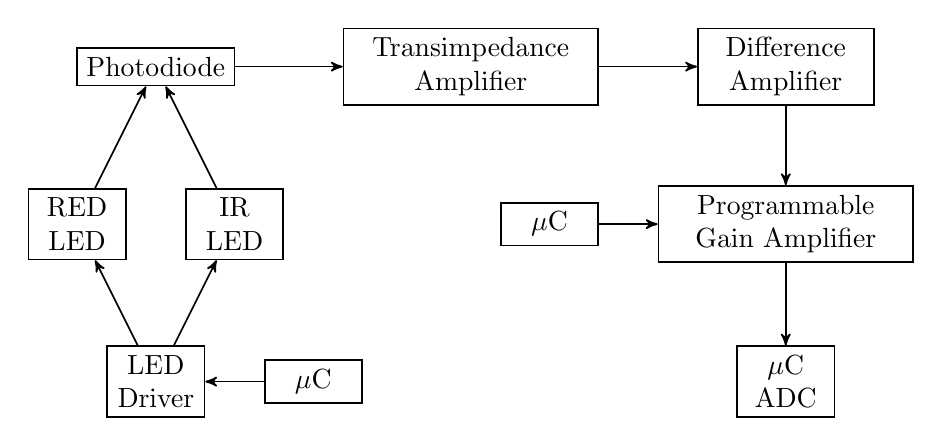
\begin{tikzpicture}
		[->,>=stealth',semithick]	
		\node[rectangle,draw] (r0) at (0, 0) {Photodiode};
		\node[rectangle,draw,text width=1cm, align=center] (r1) at (-1, -2) {RED LED};
		\node[rectangle,draw,text width=1cm, align=center] (r2) at (1, -2) {IR LED};	
		\node[rectangle,draw,text width=1cm, align=center] (r3) at (0, -4) {LED Driver};
		\node[rectangle,draw,text width=3cm, align=center] (r4) at (4, 0) {Transimpedance Amplifier};
		\node[rectangle,draw,text width=2cm, align=center] (r5) at (8, 0) {Difference  Amplifier};
		\node[rectangle,draw,text width=3cm, align=center] (r6) at (8, -2) {Programmable Gain Amplifier};
		\node[rectangle,draw,text width=1cm, align=center] (r7) at (8, -4) {$\mu$C ADC};
		\node[rectangle,draw,text width=1cm, align=center] (r8) at (2, -4) {$\mu$C};
		\node[rectangle,draw,text width=1cm, align=center] (r9) at (5, -2) {$\mu$C};
		
		\path (r1) edge (r0);
		\path (r2) edge (r0);
		\path (r3) edge (r1) 
		edge (r2);
		\path (r0) edge (r4);
		\path (r4) edge (r5);
		\path (r5) edge (r6);
		\path (r6) edge (r7);
		\path (r8) edge (r3);
		\path (r9) edge (r6);
		
	\end{tikzpicture}
	\caption{System Block Diagram}
	\end{figure}

	Referring the Block diagram, subsections are divided below that show the circuit and corresponding oscilloscope trace outputs.
	
	\subsection{Front End}	
	
		\subsubsection{Transimpedance Stage}
		
			Photodiode's current is needed to be converted to a proportional voltage so that ultimately the microcontoller can convert the voltage to a digital value using an ADC for calculation of SpO\textsubscript{2}. A simple Transimpedance Amplifier configuration was used to achieve this:
			
			\begin{figure}[ht!]\centering
				\begin{circuitikz}[american] 
					\draw
					
					(2,3) node[op amp,yscale=-1] (opamp) {}
					(opamp.down) -- +(0,0.3) node[vcc]{Vcc}
					(opamp.up) -- +(0,-0.3) node[ground]{}
					(0,0) node[ground]{} to[pDo, l^=$D$, f^=$I$]  (0,2.5) to (opamp.-)
					(opamp.+) node[ground]{}
					(opamp.-) -- ++(0,-1.7) -- ++(0.5,0)
					to [R, l^=$R_1$] ++(1.5,0) -- ++(0.4,0) to (opamp.out)
					(opamp.-)  ++(0,-1.7) -- ++(0,-1.3) -- ++(0.5,0) 
					to [C, l^=$C_1$]  ++(1.5,0) -- ++(0.4,0) -- ++(0,1.3) 
					(opamp.out) -- ++(1,0) to [open,v=$V_1$,o-o] ++(0,-3) node[ground]{};
					
				\end{circuitikz}
			\end{figure}
			
		
			As per led's intensity, if a current of 10$\mu$A is produced in the photodiode, and R = 100K$\Omega$, according to Ohm's law, $V_1$ = 1 V. Capacitor is used for low-pass filtering of the pulse. Cut off frequency would be:
		
		
			\begin{equation}	
				F_c = \frac{1}{2\pi R_1C_1}
			\end{equation}
		
			If R\textsubscript{1}=576K$\Omega$, C\textsubscript{1} = 33pF, 
			
			\[	
			F_c \approx \SI{8.3}{\kilo\hertz}
			\]
		
			\begin{figure}[ht!]
				\centering
				\subfloat[V\textsubscript{1} 
				]{\includegraphics[width=0.9\textwidth]{../common/circuit/itov.png}}
				\hfill
				\subfloat[V\textsubscript{1} zoomed in 
				]{\includegraphics[width=0.9\textwidth]{../common/circuit/itov_zoom.png}
				\label{fig:itov}}
				\caption{V\textsubscript{1} Oscilloscope trace (Red \& IR pulsed sequentially) }
			\end{figure}
		
			Since LEDs are pulse on-off at a fast rate sequentially the pulse would look like a square wave. We need to use a pulse frequency less than 1/10\textsuperscript{th} of this cut-off to pulse the LEDs so that the square wave with all its high-frequency components is clearly visible and not filtered out.
			
			\[	
			F_p = \SI{500}{\hertz}
			\]
					
		
			It can be seen in traces, 2 PPG signals are observable, riding on a DC level. Higher amplitude one is a result of ir led pulsing, while lower amplitude is from red led. Since the peaks correspond to heart rate, in this case as per trace, it measures out to be 1.42/sec or 85BPM. Individual pulses which construct the signal can be seen in Figure \ref{fig:itov}. Amplitude of detected red signal is lower than ir and that is due to:
			
			\begin{itemize}
				
				\item Higher intensity of ir led due to higher ir current.
				\item Photodiode's red sensitivity is 80\% of ir sensitivity. 
				\item Ir penetrates into skin deeper than red, hence a better ir response is visible at photodiode\cite{penetrate}.
				
			\end{itemize}		
			Hence to obtain a suitable response, it is important to increase led intensity until it reaches a required level so that the PPG signal has a higher amplitude.	
			
		\subsubsection{Difference Amplifier}
		
			PPG signal needs to be amplified to a suitable level so that full scale ADC range can be utilized to better digitize the signal. Right now, amplitude of PPG signal is quite low and DC level is higher. We are not bothered by the DC anymore, $\mu$C can read it and store for R value calculation, we only need to amplify the AC part which is an envelope of the signal. Direct amplification would lead to gain of the DC level as well, as the required signal is riding on top of it. This will saturate the opamp and amplification level range will be quite low. 
			
			\begin{figure}[ht!]
				\centering
				\includegraphics[width=0.8\textwidth]{../common/circuit/diff.png}
				\caption{Effect of Difference Amplifier}
				\label{fig:diff}
			\end{figure}	
			
			If we can subtract the DC level from entire signal, only AC would remain which can be easily amplified further at higher levels. A Difference amplifier along with a 8bit Digital to analog converter (DAC) generating the DC cancellation signal can be used here. Since red and ir have different levels, separate DC levels are generated by DAC in sync with the pulsed frequency.\medskip 
			
			As shown in Figure \ref{fig:diff} a plot generated in Octave demonstrates subtraction of required signal and diff signal. This difference can then be amplified further. Pulse width of diff signal is slightly larger than required signal so that there are no spikes on edges in output signal. Also the lower level of diff signal is slightly above 0V to allow the difference to always be negative in low states and since negative supply is grounded, output would be 0V here.
			
			\begin{figure}[ht!]\centering
				\begin{circuitikz}[american] 
					\draw
					
					(4,3) node[op amp,yscale=-1] (opamp) {}
					(opamp.down) -- +(0,0.3) node[vcc]{Vcc}
					(opamp.up) -- +(0,-0.3) node[ground]{}
					(opamp.-) to [R, l^=$R_1$] ++(-2,0) node[label={left:$V_{dac1}$}] {}
					(opamp.+) to [R, l^=$R_1$] ++(-2,0) node[label={left:$V_1$}] {}
					(opamp.+) to [R, l^=$R_1$] ++(0,2) node[ground,rotate = 90]{}
					(opamp.-) -- ++(0,-1.7) -- ++(0.5,0)
					to [R, l^=$R_1$] ++(1.5,0) -- ++(0.4,0) to (opamp.out)
					(opamp.out) -- ++(1,0) to [open,v=$V_2$,o-o] ++(0,-3) node[ground]{};
			
				\end{circuitikz}
			\end{figure}
			


			\[
				V_2 = \frac{R_1}{R_1}(V_1 - V_{dac1})
			\]
			
			
			For $R_1 = 10K$,
			
			\[
				V_2 \approx V_1 - V_{dac1}
			\]
			
						
		\subsubsection{Programmable Gain Amplifier}
		
			It becomes necessary to amplify the signal as skin tone, improper finger contact with sensor or any skin pigmentation\cite{skin} can cause attenuation in signal leading to low amplitudes. This stage provides selectable variable gain which can be set by microcontroller.
			
			$\mu$C would determine what level of further amplification is required and drive the respective pin high so that resistor value would get selected.
			
			
			\begin{figure}[ht!]\centering
				\begin{circuitikz}[american] 
					\draw
						(2,3) node[op amp,yscale=-1] (opamp) {}
						(opamp.down) -- +(0,0.3) node[vcc]{Vcc}
						(opamp.up) -- +(0,-0.3) node[ground]{}
						(opamp.+) to ++(-2,0) node[label={left:$V_2$}] {}
						(opamp.-) -- ++(0,-1.7) -- ++(1,0)
						to [R, l^=$10K$] ++(1,0) -- ++(1,0) -- ++(0,2.2) to (opamp.out)
						(opamp.-) ++(0,-1.7) -- ++(0,-1.5) to [R, l^=$10K$] ++(0,-1) -- ++(0,-0.5)
						++(0,-0.5) node[npn] (Q1){}
						(Q1.E) node[ground]{}
						(Q1.B) to [R, l^=$4.7K$] ++(-1.5,0) node[label={left:S1}] {}
						
						(opamp.-) ++(0,-1.7) ++(0,-0.75) -- ++(3.5,0) -- ++(0,-0.75)		
						to [R, l^=$4.7K$] ++(0,-1) -- ++(0,-0.5)
						++(0,-0.5) node[npn] (Q2){}	
						(Q2.E) node[ground]{}	
						(Q2.B) to [R, l^=$4.7K$] ++(-1.5,0) node[label={left:S2}] {}
						
						(opamp.-) ++(0,-1.7) ++(0,-0.75) ++(2,0) -- ++(5,0) -- ++(0,-0.75)		
						to [R, l^=$2.35K$] ++(0,-1) -- ++(0,-0.5)
						++(0,-0.5) node[npn] (Q3){}	
						(Q3.E) node[ground]{}	
						(Q3.B) to [R, l^=$4.7K$] ++(-1.5,0) node[label={left:S3}] {};
						
						
				 \end{circuitikz}
			\end{figure}	
	
			\begin{center}
				\begin{tabular}{ |c|c|} 
					\hline
					\textbf{Switch} & \textbf{Gain}   \\ 
					\hline
					all off & 1 	\\ 
					\hline
					S1 & 2  		\\ 
					\hline
					S2 & 3  		\\ 
					\hline
					S1+S2 & 4  		\\ 
					\hline
					S3 & 5  		\\ 
					\hline
					S1+S3 & 6	  	\\ 
					\hline
					S2+S3 & 7  		\\ 
					\hline
				\end{tabular}
			\end{center}
		
	
	\subsection{LED Driver}

	
		As discussed previously, the detected signal levels can be very low after I to V stage. LED Driver needs to increase current to the leds as required. Following circuit is used as a voltage controlled current source, voltage is set by the DAC as instructed by the $\mu$C.
		
		\begin{figure}[ht!]\centering
			\begin{circuitikz}[american] 
				\draw
				
				(4,3) node[npn] (Q1){}
				(Q1.E) to [R, l^=20] ++(0,-1.5) node[ground]{}
				(Q1.B) to [R, l^=4.7K] ++(-1.5,0) node[label={left:$V_{dac2}$}] {}
				(Q1.C) -- ++(-1,0) -- ++(0,0.5) ++(0,0.5)  node[npn] (Q2){}
				(Q2.B) to [R, l_=10K] ++(-1.5,0) node[label={left:Red pulse}] {}
				(Q2.C) -- ++(0,1) node[]{} ++(0,0.2) node[]{Red cathode}
				(Q1.C) -- ++(1,0) -- ++(0,0.5) ++(0,0.5) node[npn,xscale=-1] (Q3){}
				(Q3.B) to [R, l^=10K] ++(1.5,0) node[label={right:IR pulse}] {}
				(Q3.C) to ++(0,1) node[]{} ++(0,0.2) node[]{Ir cathode};
			\end{circuitikz}
		\end{figure}
		
		
		Leds get activated by a single bridge configuration, whenever red/ir pulse is active, corresponding red/ir leds get active (led anodes connected to Vcc). Amount of current would depend on $V_{dac2}$ \& $R_1$.
		
		$V_{dac2}$ is also set individually for red and ir as per the pulsed frequency. If intensity is not sufficient for signal detection, it is necessary to increase $V_{dac2}$. $\mu$C would determine the thresholds and modulate the control voltage accordingly.
	
		Shown below is final output after the PGA stage.
		The gained up PPG signal is clearly visible for both red and ir which is at a suitable level for ADC capture and usage in algorithms for calculations.
	
	
	\begin{figure}[ht!]
		\centering
		\subfloat[Final output - green, V\textsubscript{1} - blue
		]{\includegraphics[width=1\textwidth]{../common/circuit/final_out.png}}
		\hfill
		\subfloat[Final output measurement
		]{\includegraphics[width=1\textwidth]{../common/circuit/final_out_meas.png}}
		\caption{Final output}
	\end{figure}		
		
	\section{Algorithm}
	
	\begin{figure}[ht!]
		\hspace*{-1.8cm}
		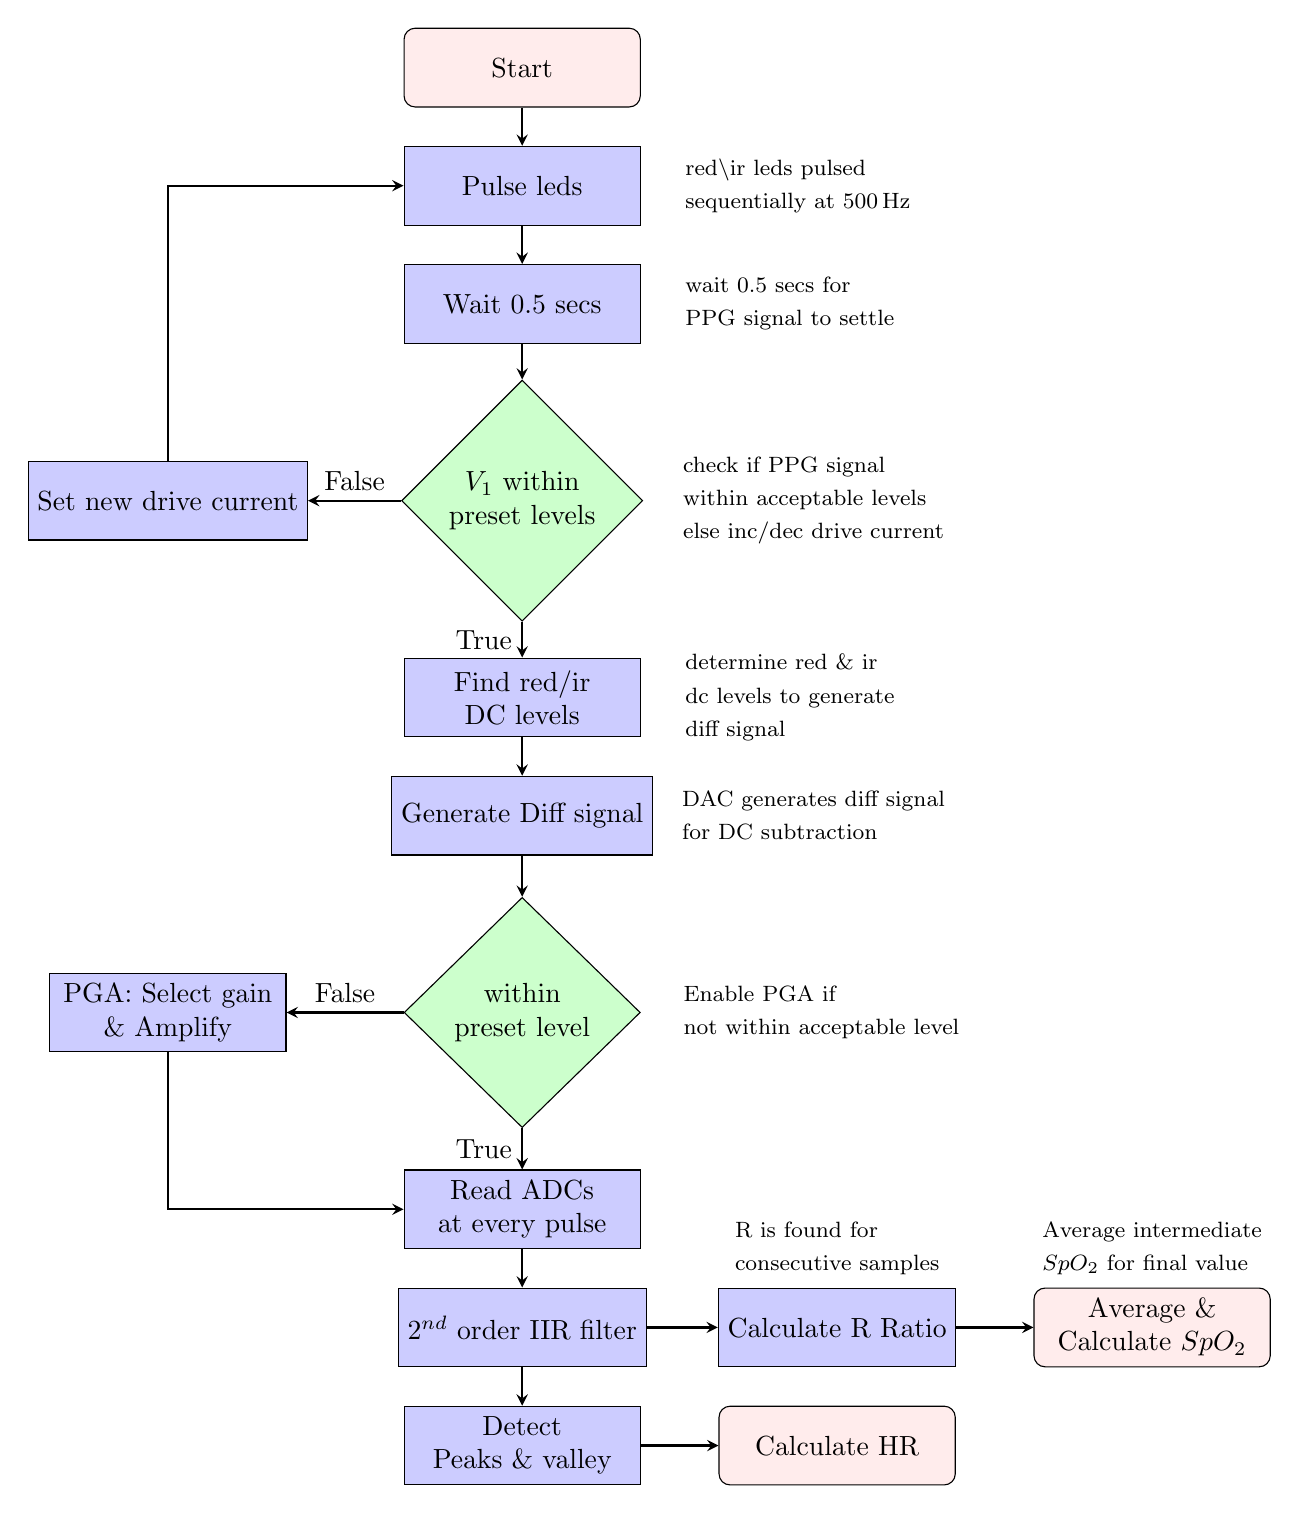
\begin{tikzpicture}
			[node distance=1.5cm]
			
			\tikzstyle{startstop} = [rectangle, rounded corners, minimum width=3cm, minimum height=1cm,text centered, draw=black, fill=pink!30,align = center]
			
			\tikzstyle{io} = [trapezium, trapezium left angle=70, trapezium right 	angle=110, minimum width=3cm, minimum height=1cm, text centered, draw=black]
			
			\tikzstyle{process} = [rectangle, minimum width=3cm, minimum height=1cm, text 	centered, draw=black,align = center, fill = blue!20]
			
			\tikzstyle{decision} = [diamond, minimum width=3cm, minimum height=1cm, 
			align = center, draw=black, fill = green!20]
						
			\tikzstyle{arrow} = [thick,->,>=stealth]

			\node (st) [startstop] {Start};
			\node (pls) [process,below of=st] {Pulse leds};
			\node (wt) [process, below of=pls] {Wait 0.5 secs};
			\node (findlv) [decision, below of=wt,yshift=-1cm] {$V_1$ within\\preset levels};
			\node (setlv) [process, left of=findlv,xshift=-3cm] {Set new drive current};
			\node (dc) [process, below of=findlv,yshift=-1cm] {Find red/ir \\DC levels};
			\node (diff) [process, below of=dc] {Generate Diff signal};
			\node (amp) [decision, below of=diff,yshift=-1cm] {within\\ preset level};
			\node (pga) [process, left of=amp,xshift=-3cm] {PGA: Select gain\\ \& Amplify};
			\node (adc) [process, below of=amp,yshift=-1cm] {Read ADCs\\at every pulse};
			\node (filt) [process, below of=adc] {$2^{nd}$ order IIR filter};
			\node (peaks) [process, below of=filt] {Detect \\Peaks \& valley};
			\node (hr) [startstop,right of=peaks,xshift=+2.5cm] {Calculate HR};
			\node (ratio) [process,right of=filt,xshift=+2.5cm] {Calculate R Ratio};
			\node (spo2) [startstop,right of=ratio,xshift=+2.5cm] {Average \& \\Calculate $SpO_2$};
			
			\draw [arrow] (st) -- (pls);
			\draw [arrow] (pls) -- (wt);
			\draw [arrow] (wt) -- (findlv);
			\draw [arrow] (findlv) -- node [above]{False} (setlv);
			\draw [arrow] (setlv) |- (pls);
			\draw [arrow] (findlv) -- node [left]{True} (dc);
			\draw [arrow] (dc) -- (diff);
			\draw [arrow] (diff) -- (amp);
			\draw [arrow] (amp) -- node [above]{False} (pga);
			\draw [arrow] (amp) -- node [left]{True} (adc);
			\draw [arrow] (pga) |- (adc);
			\draw [arrow] (adc) -- (filt);
			\draw [arrow] (filt) -- (peaks);
			\draw [arrow](peaks) -- (hr);
			\draw [arrow](filt) -- (ratio);
			\draw [arrow](ratio) -- (spo2);		
		
			\draw (pls) ++(3.5,0) node [align = left]{\footnotesize
			red$\backslash$ir leds pulsed\\
			\footnotesize sequentially at $\SI{500}{\hertz}$};
			
			\draw (wt) ++(3.4,0) node [align = left]{\footnotesize
				wait 0.5 secs for\\\footnotesize PPG signal to settle};
			
			\draw (findlv) ++(3.7,0) node [align = left]{\footnotesize
				check if PPG signal\\\footnotesize within acceptable levels\\
				\footnotesize else inc/dec drive current};
			
			\draw (dc) ++(3.4,0) node [align = left]{\footnotesize
				determine red \& ir \\\footnotesize dc levels to generate\\
				\footnotesize diff signal};
			
			\draw (diff) ++(3.7,0) node [align = left]{\footnotesize
				DAC generates diff signal\\\footnotesize for DC subtraction};
			
			\draw (amp) ++(3.8,0) node [align = left]{\footnotesize
				Enable PGA if\\\footnotesize not within acceptable level};
			
			\draw (ratio) ++(0,1) node [align = left]{\footnotesize
				R is found for\\\footnotesize consecutive samples};
			\draw (spo2) ++(0,1) node [align = left]{\footnotesize
				Average intermediate\\\footnotesize $SpO_2$ for final value};	
			
		\end{tikzpicture}
		\caption{Program Flow}
	\end{figure}
	
	\subsection{IIR Filter}

		ADC read samples can have little noise spikes which if passed directly to peak-valley detect function will lead to a lot of false detection and every peak-valley will not be captured accurately. A 2\textsuperscript{nd} order IIR filter is sufficient to smooth out the spikes before starting with estimations. Below is a 2\textsuperscript{nd} order IIR transfer function as difference equation:
		
		\[
		y_i = b_1*x_i + b_2*x_{i-2} - a_2*y_{i-1} + b_3*x_{i-1} - a_3*y_{i-2}
		\]
		
		where,
		
		$y_i$: current output
		
		$x_{i-1}$: previous input
		
		$y_{i-1}$: previous output
		
		$y_{i-2}$: output previous to $y_{i-1}$
		
		$x_i$: current input
		
		$x_{i-2}$: input previous to $x_{i-1}$
		
		
		\begin{figure}[ht!]
			\centering
			\includegraphics[width=0.75\textwidth]{../common/algo/filter.png}
			\caption{2\textsuperscript{nd} order butterworth IIR filter}
			\label{fig:filter}
		\end{figure}
		
		Octave's $butter$ function\footnote{\url{https://octave.sourceforge.io/signal/function/butter.html}} was used to get the transfer function coefficients for a low pass configuration. Sampling frequency of 500Hz and a cut-off 3.3Hz (for max HR of 200) was used. Calculated below are the coefficient values:
		
		$a_2 = -1.94137, a_3 = 0.94304$
		
		$b_1 = b_3 = 4.1762e-04$
		
		$b_2 = 8.3523e-04$
		
		To visualize filter's performance, a raw signal was captured from ADC, filter equation was implemented and applied on the input signal in Octave. As seen in Figure \ref{fig:filter} filter is quite effective in suppressing noise and produces a smooth output\footnote{Only a 1\textsuperscript{st} order filter was implemented in actual program as it worked "just fine", but it is much better to have a 2\textsuperscript{nd} order filter for suitable filtering performance.}.
		
	
	\subsection{Heart Rate}
	
		HR is calculated using mountaineer's method for peak detection (MMPD) in photoplethysmographic signals\cite{mmpd}.
		
		In this method, slope is calculated for every sample and as slope changes from positive to negative, sample will corresponding to a peak. Similarly a slope change from negative to positive would be a valley. A count for positive or negative consecutive slopes is also taken and compared with a preset value which updates with every detected peak to improve the robustness of the algorithm. A timer running would store peak timings and time difference between consecutive peaks would correspond to the heart rate. Shown below is a visualization of the algorithm ran on a sample set. Peaks \& valleys are captured quite accurately.
		
		\begin{figure}[ht!]
			\centering
			\includegraphics[width=0.7\textwidth]{../common/algo/mmpd.png}
			\caption{HR Algorithm applied to sample data}
		\end{figure}
	
	\subsection{SpO\textsubscript{2} Calculation}
		
		As discussed previously in equation \eqref{eq:calc}:
		
		
		\[
			R = \sfrac{\frac{V_{p2} - V_{l2}}{DC_2}}{\frac{V_{p1} - V_{l1}}{DC_1}}
		\]	
		
		We don't want to use signal's actual peak and valleys for R calculation as that is dependent on heart rate and any averaging of values on top of that would delay the final SpO\textsubscript{2}\% which we intend to obtain. Hence a weight averaging method is used\cite{wuk}, where instantaneous SpO\textsubscript{2}\% is calculated for neighboring samples and averaged together. This ensure multiple instantaneous values are obtained which can be averaged to obtain a final value. Following steps are performed in order:
				
		\begin{figure}[ht!]
			\centering
			\includegraphics[width=0.5\textwidth]{images/spo2_algo.png}
			\caption{Selecting samples for instantaneous SpO\textsubscript{2}}
		\end{figure}
	
		\begin{enumerate}
			\item Find R between consecutive samples of red and ir signals: $S_{i+1}$ \& $S_{i}$. 
			
			\[
			R = \sfrac{\frac{S_{i_2+1} - S_{i2}}{DC_2}}{\frac{S_{i_1+1} - S_{i1}}{DC_1}}
			\]	
			
			Find SpO\textsubscript{2} with this R value which can obtained using a typical relationship curve equation as shown in Figure \ref{fig:curve}:
			\[		
				SpO_2 = -25*R + 110;
			\]
			\item Assign a weight to this SpO\textsubscript{2} based on the current average. If this instantaneous SpO\textsubscript{2} is lower than average, assign a lower weight. If nearer to average, assign a higher weight.
			
			\item Once weights are assigned for 20 samples, calculate a weighted average. Store this weighted average.
			
			\item Restart at step 1 and perform 10 such iterations.
			\item After 10 iterations, average the calculated weighted averages in each iteration. This becomes the final SpO\textsubscript{2}. Update this value with the current SpO\textsubscript{2} average which is used for assigning weights.
		\end{enumerate}
			
		A detailed explanation of this algorithm is in - Pulse Oximetry: Analysis of Theory, Technology and Practise\cite{wuk}
		
		Finally, an OLED display is refreshed every 5 secs with SpO\textsubscript{2}\% \& HR value.
		

	\section{पीसीबी व एन्क्लोज़र}

	\subsection{पीसीबी}	
	
		\begin{figure}[ht!]
			\centering
			\includegraphics[width=0.6\textwidth]{../common/pcb/pcb.png}
			\caption{पूर्ण पीसीबी}
		\end{figure}


		\begin{figure}[ht!]
			\centering
			\subfloat[पीसीबी पिछ्ला भाग
			]{\includegraphics[width=0.5\textwidth]{../common/pcb/pcb_back.png}}
			\hfill
			\subfloat[पीसीबी अग्र भाग
			]{\includegraphics[width=0.5\textwidth]{../common/pcb/pcb_front.png}}
			\caption{पीसीबी के चित्र}
		\end{figure}

		पीसीबी डिजाइन को 2 परतों पर पूरा किया गया था जिसमें अधिकांश अंशो को पीछे की तरफ रखा गया था ताकि उन्हें डोसा पैन पर आसानी से री-फ़्लो किया जा सके। सामने की तरफ के सभी अंशो को हाथ से सोल्डर किया जाना है। 

		\begin{itemize}
			
			\item डिवाइस को संचालित करने के लिए एक सॉफ्ट लैच पावर ऑन/ऑफ स्विच सर्किट भी शामिल है।
			
			\item UPDI इंटरफ़ेस के माध्यम से $\mu$C को प्रोग्राम करने के लिए एक प्रोग्रामिंग हेडर भी लगाया गया था।
			
			\item Led, बैटरी और फोटोडायोड को जोड़ने के लिए कनेक्शन हेडर बनाये गए है जो एन्क्लोज़र के निचले हिस्से पर मौजूद होंगे।
			
			\item OLED डिस्प्ले के लिये हैडर। 

		\end{itemize}
	
		जांच के लिए आसान पहुंच और ऑसिलोस्कोप पर संकेतों को देखने के लिए सामने की तरफ पर्याप्त परीक्षण बिंदु जोड़े गए थे।
		
		पीसीबी साइज को OLED डिस्प्ले मॉड्यूल के बराबर रखने के लिए 0402 साइज रेसिस्टर्स/कैपेसिटर का इस्तेमाल किया गया।
					

	\subsection{एन्क्लोज़र}		
		
		एन्क्लोज़र को एक सरल ऑक्सीमीटर से संदर्भ लेते हुए डिज़ाइन किया गया था जिसमें शीर्ष पर डिस्प्ले \& PCB, निचला भाग पर फिंगर इंसर्ट और बैटरी कंपार्टमेंट है।
		
		\begin{figure}[ht!]
			\centering
			\includegraphics[width=0.5\textwidth]{../common/enc/enc.png}
			\caption{पूर्ण एन्क्लोज़र}
		\end{figure}	
				
		उपरि भाग पर फोटोडायोड और निचले में led एक चिंतनशील सेट अप मे मौजूद है। 
				
		\begin{figure}[ht!]
			\centering
			\subfloat[फोटोडायोड कम्पार्टमेंट
			]{\includegraphics[width=0.45\textwidth]{../common/enc/top_base.png}}
			\hfill
			\subfloat[पीसीबी के लिए स्पेसर
			]{\includegraphics[width=0.45\textwidth]{../common/enc/top_base2.png}}
			\caption{उपरि भाग}
		\end{figure}
	
	
		\begin{figure}[ht!]
			\centering
			\subfloat[बैटरी कम्पार्टमेंट
			]{\includegraphics[width=0.45\textwidth]{../common/enc/bot_base.png}}
			\hfill
			\subfloat[Led कम्पार्टमेंट
			]{\includegraphics[width=0.45\textwidth]{../common/enc/bot_base2.png}}
			\caption{निचला भाग}
		\end{figure}
	
		उंगली को सुरक्षित करना एक महत्वपूर्ण हिस्सा है क्योंकि किसी भी तरह के डगमगाने या अनुचित संपर्क से सिग्नल की गुणवत्ता और गणना किए गए मापदंडों में गिरावट आ सकती है। उंगली पर एक मजबूत दबाव प्राप्त करना जरुरी है जो इसे स्थिर रखेगा, इसीलिये रोटेशन तंत्र में एक सेफ्टीपिन (क्लिप भाग को हटाकर) का उपयोग किया गया है।
		
		\begin{figure}[ht!]
			\centering
			\subfloat[सेफ्टीपिन
			]{\includegraphics[width=0.5\textwidth]{../common/enc/pin.png}}
			\hfill
			\subfloat[सेफ्टीपिन का द्र्शय
			]{\includegraphics[width=0.5\textwidth]{../common/enc/pin_side.png}}
			\caption{सेफ्टीपिन निचले भाग मे}
		\end{figure}	
		
		निष्क्रिय स्थिति में, सेफ्टीपिन (पिन) प्राकृतिक गैर-विस्तारित अवस्था में होगा इसलिए दोनों  भाग बंद हो जाएंगे। जब उंगली डाली जायेगी, उपरि हिस्से को उठना होगा रोटेशन तंत्र के माध्यम से जभी उंगली अंदर जाएगी। इस से पिन उपरी भाग को उंगली पर नीचे धकेलेगा जिससे फोटोडायोड के साथ अच्छा संपर्क सुनिश्चित होगा और एक मजबूत पकड़ बनेगी। 

		\begin{figure}[ht!]
			\centering
			\includegraphics[width=0.6\textwidth]{../common/enc/snap.png}
			\caption{स्नैप फिट क्रॉस-सेक्शन}
		\end{figure}	
		
	
		स्नैप फिट तत्वों को लागू किया गया है जिससे जब भी आवश्यक हो कवर भागों को फिट करना और निकालना आसान हो सके। 
	
	\pagebreak
	
	
	\begin{thebibliography}{10}		
		
		
		\bibitem{light}
		Hartmann Vera, Liu Haipeng.
		\textit{Quantitative Comparison of Photoplethysmographic 
		Waveform Characteristics: Effect of Measurement Site}
		Frontiers in Physiology , vol 10 (2019)
		\url{https://www.frontiersin.org/article/10.3389/fphys.2019.00198}

		\bibitem{penetrate}
		Ash, Caerwyn et al.
		\textit{Effect of wavelength and beam width on 
		penetration in light-tissue interaction using computational methods.}
		Lasers in medical science vol. 32,8 (2017): 1909-1918.
		\url{https://www.ncbi.nlm.nih.gov/pmc/articles/PMC5653719/}		
		
		\bibitem{skin}
		Feiner, John R. MD, Severinghaus.
		\textit{Dark Skin Decreases the Accuracy of Pulse Oximeters at 
		Low Oxygen Saturation}
		December 2007 - Volume 105 - Issue 6 - p S18-S23
		\url{https://journals.lww.com/anesthesia-analgesia/Fulltext/2007/12001/Dark_Skin_Decreases_the_Accuracy_of_Pulse.4.aspx}		
		
		\bibitem{mmpd} 
		Argüello-Prada, Erick Javier. 
		\textit{The mountaineer's method for peak detection in photoplethysmographic signals.} 
		Revista Facultad De Ingenieria-universidad De Antioquia 2018 (2019): 42-50
		\url{https://api.semanticscholar.org/CorpusID:116767900}
		 
		\bibitem{nxp} 
		Santiago Lopez, Freescale Semiconductor.
		\textit{Pulse Oximeter Fundamentals and Design} 
		Document Number: AN4327, Rev. 2, 11/2012
		\url{https://www.nxp.com/docs/en/application-note/AN4327.pdf}
		
		\bibitem{ti}
		Praveen Aroul, Texas Instruments.
		\textit{Miniaturized Pulse Oximeter Reference Design}
		User’s Guide and Test Report TIDA-00311
		\url{https://www.ti.com/lit/pdf/tidu542}
		
		\bibitem{micro}
		Zhang Feng, Microchip Technology Inc.
		\textit{Pulse Oximeter Design Using Microchip’s Analog Devices
		and dsPIC® Digital Signal Controllers (DSCs)}
		AN1525,   04/28/2015
		\url{http://ww1.microchip.com/downloads/en/Appnotes/00001525B.pdf}

		\bibitem{oxf}
		Dr. Neil Townsend, Department of Engineering Science, University of Oxford.
		\textit{C3B Medical Electronics Lecture Notes}
		\url{https://www.robots.ox.ac.uk/~neil/teaching/lectures/med_elec/notes6.pdf}	

		\bibitem{wuk}
		Michael W. Wukitsch, BA,Michael T. Petterson.
		\textit{Pulse Oximetry: Analysis of Theory,Technology and Practice}
		\url{https://doi.org/10.1007/BF01617328}	
	\end{thebibliography}

	\pagebreak
	\section{Closing Comments}
	
	I referred the listed documents extensively throughout the process specifically \cite{nxp}, \cite{ti}, \cite{micro}, \cite{oxf}, \cite{wuk} to close gaps in my understanding and to improve/revisit the design.\par
	\bigskip
	Completing this project taught me lot of things from a design perspective and a lot of respect for the products that I use on daily basis considering the amount of iterations something must have went through and enormous number of checks/edge cases to ensure it works just right.
	
	For me, this project took close to 7 months for completion, considering I worked 20hrs/week on average. I made 3 iterations in total during this timeline, documented is the 3\textsuperscript{rd} version. There are still a lot of improvements i can think of hence a shortcomings/recommended improvements page is added to project directory where i have listed all further improvements or current issues which can be worked on. I wouldn't want to progress these anymore as somewhere i feel the initial goal with which i started off has met:
	
	\begin{itemize}
		\item Making something from scratch(at least a suitable prototype) and documenting the entire project in 2 different languages.
		\item A YouTube Vlog of the project.
	\end{itemize}

	I hadn't done any of this in the past hence this project required me to change myself to accomplish it. Most important lessons that i have learned from this journey are:
	
	\begin{itemize}
	\item Never let something which appears difficult or out of reach contemplate your decision to work on it. You know nothing so everything is going to be difficult to understand but it shouldn't become a filter for choosing what to work on.
	
	\item Consistency. There were many issues with design that I found on weekends which later got resolved in the next weekend only because there was consistency and I was involved with the problem on a daily basis performing new workarounds every day.
	\end{itemize}

	\bigskip
	I would end this document now. If you have any suggestions or comments, you can reach me out on Twitter
	\href{https://twitter.com/yskabhijeet}{@yskabhijeet}.
	

	
\end{document}
